\documentclass[12pt,letterpaper]{exam}
\usepackage[lmargin=1in,rmargin=1in,tmargin=1in,bmargin=1in]{geometry}
\usepackage{../style/exams}

% -------------------
% Course & Exam Information
% -------------------
\newcommand{\course}{MATH 115: Exam 1}
\newcommand{\term}{Fall --- 2024}
\newcommand{\examdate}{09/09/2024}
\newcommand{\timelimit}{75 Minutes}

\setbool{hideans}{false} % Student: True; Instructor: False


% -------------------
% Content
% -------------------
\begin{document}

\examtitle
\instructions{Write your name on the appropriate line on the exam cover sheet. This exam contains \numpages\ pages (including this cover page) and \numquestions\ questions. Check that you have every page of the exam. Answer the questions in the spaces provided on the question sheets. Be sure to answer every part of each question and show all your work. If you run out of room for an answer, continue on the back of the page --- being sure to indicate the problem number.} 
\scores
\bottomline
\newpage


% -------------------
% Questions
% -------------------
\begin{questions}

% Question 1
\newpage
\question Let $A= [-4, 5]$, $B= (-5, 2]$, $C= [2, 6)$, and $D= (-2, 2)$. Compute the following sets: \pvspace{0.5cm}
	\begin{parts}
	\part[3] $A \cap B$ \vfill
		\[
		A \cap B= [-4, 2]
		\] \vfill
	
	\part[3] $D \cup C$ \vfill
		\[
		D \cup C= (-2, 6)
		\] \vfill
	
	\part[4] $(B \cup D) \cap A$ \vfill
		\[
		(B \cup D) \cap A= [-4, 2]
		\] \vfill
	\end{parts}

\sol{
	\[
	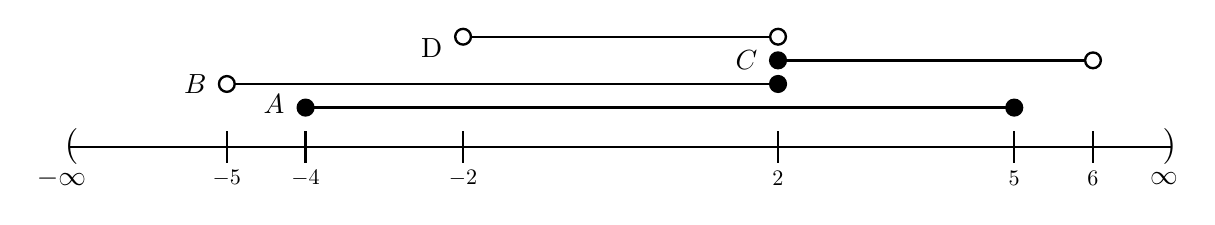
\begin{tikzpicture}
	\draw[line width=0.03cm] (-7,0) -- (7,0); % Main Line
	\node at (-6.97,0) {\scalebox{1.3}{$\mathbf ($}}; \node at (6.97,0) {\scalebox{1.3}{$\mathbf )$}}; % Ends
	\node at (-7.1,-0.4) {$-\infty$}; \node at (6.9,-0.4) {$\infty$}; % \pm Infinity
	% A
	\draw[line width=0.03cm] (-4,0.50) -- (5,0.50);
	\draw[line width=0.03cm,fill=black] (-4,0.50) circle (0.1);
	\draw[line width=0.03cm,fill=black] (5,0.50) circle (0.1);
	\node at (-4.4,0.55) {$A$};
	% B
	\draw[line width=0.03cm] (-5,0.8) -- (2,0.8);
	\draw[line width=0.03cm,fill=white] (-5,0.8) circle (0.1);
	\draw[line width=0.03cm,fill=black] (2,0.8) circle (0.1);
	\node at (-5.4,0.8) {$B$};
	% C
	\draw[line width=0.03cm] (2,1.1) -- (6,1.1);
	\draw[line width=0.03cm,fill=black] (2,1.1) circle (0.1);
	\draw[line width=0.03cm,fill=white] (6,1.1) circle (0.1);
	\node at (1.6,1.1) {$C$};
	% D
	\draw[line width=0.03cm] (-2,1.4) -- (2,1.4);
	\draw[line width=0.03cm,fill=white] (-2,1.4) circle (0.1);
	\draw[line width=0.03cm,fill=white] (2,1.4) circle (0.1);
	\node at (-2.4,1.25) {D};
	
	% Labels
	\draw[line width=0.03cm] (-5,-0.2) -- (-5,0.2); \node at (-5,-0.4) {\scalebox{0.8}{$-5$}}; % -5
	\draw[line width=0.03cm] (-4,-0.2) -- (-4,0.2); \node at (-4,-0.4) {\scalebox{0.8}{$-4$}}; % -4
	\draw[line width=0.03cm] (-2,-0.2) -- (-2,0.2); \node at (-2,-0.4) {\scalebox{0.8}{$-2$}}; % -2
	\draw[line width=0.03cm] (2,-0.2) -- (2,0.2); \node at (2,-0.4) {\scalebox{0.8}{$2$}}; % 2
	\draw[line width=0.03cm] (5,-0.2) -- (5,0.2); \node at (5,-0.4) {\scalebox{0.8}{$5$}}; % 5
	\draw[line width=0.03cm] (6,-0.2) -- (6,0.2); \node at (6,-0.4) {\scalebox{0.8}{$6$}}; % 6
	\end{tikzpicture}
	\]
}



% Question 2
\newpage
\question Consider the plot of a circle and points $A, B$ shown below. 
	\[
	\fbox{
	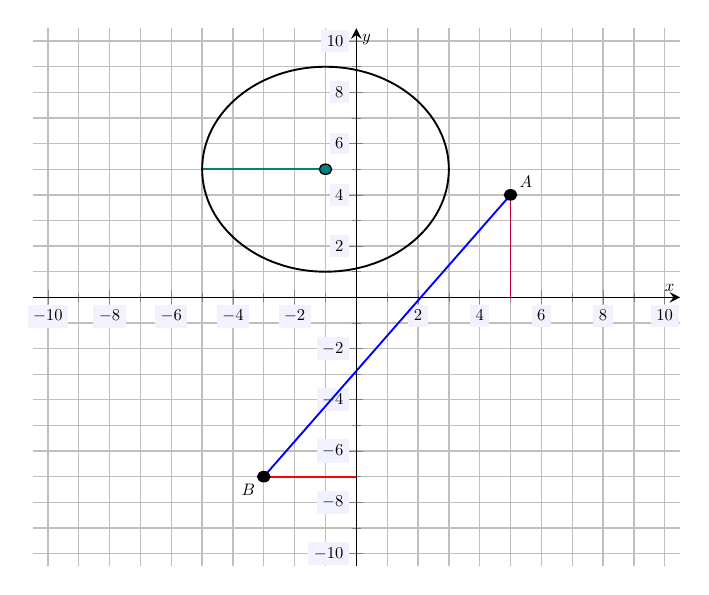
\begin{tikzpicture}[scale=1.2,every node/.style={scale=0.5}]
	\begin{axis}[
	grid=both,
	axis lines=middle,
	ticklabel style={fill=blue!5!white},
	xmin= -10.5, xmax=10.5,
	ymin= -10.5, ymax=10.5,
	xtick={-10,-8,-6,-4,-2,0,2,4,6,8,10},
	ytick={-10,-8,-6,-4,-2,0,2,4,6,8,10},
	minor tick = {-10,-9,...,10},
	xlabel=\(x\),ylabel=\(y\),
	]
	\draw[line width=0.02cm,blue] (-3,-7) -- (5,4);
	\draw[line width=0.02cm,red] (-3,-7) -- (0,-7);
	\draw[line width=0.02cm,purple] (5,4) -- (5,0);
	\draw[line width=0.02cm,teal] (-1,5) -- (-5,5);
	\draw[fill=teal] (-1,5) circle (0.2);
	
	\draw[line width=0.02cm] (-1,5) circle (4);
	\draw[fill=black] (5,4) circle (0.2); \node at (5.5,4.5) {$A$};
	\draw[fill=black] (-3,-7) circle (0.2); \node at (-3.5,-7.5) {$B$};
	\end{axis}
	\end{tikzpicture}
	}
	\] 
Based on this plot, find the following: \pspace

\begin{parts}
\part[2] The distance from $A$ to the $x$-axis. \vfill
	\[
	d(A, x\text{-axis})= 4
	\] \vfill

\part[2] The distance from $B$ to the $y$-axis. \vfill
	\[
	d(B, y\text{-axis})= 3
	\] \vfill

\part[3] The equation of the circle. \vfill
	\[
	\begin{gathered}
	\big(x - (-1) \big)^2 + (y - 5)^2= 4^2 \\[0.2cm]
	(x + 1)^2 + (y - 5)^2= 16
	\end{gathered}
	\] \vfill

\part[3] The distance between $A$ and $B$. \vfill
	\[
	d(A, B)= \sqrt{\big(5 - (-3) \big)^2 + \big(4 - (-7)^2 \big)^2}= \sqrt{8^2 + 11^2}= \sqrt{64 + 121}= \sqrt{185} \approx 13.60
	\] \vfill
\end{parts}



% Question 3
\newpage
\question Assume that $x, y, z > 0$. Showing all your work, simplify the following as much as possible: \pvspace{0.2cm}

\begin{parts}
\part[5] $\left( \dfrac{x^{-6} y z^5}{(x^{-2} z^2)^3 y^4} \right)^{-1}$ \vfill \pvspace{1cm}
	\[
	\begin{gathered}
	\left( \dfrac{x^{-6} y z^5}{(x^{-2} z^2)^3 y^4} \right)^{-1} \\[0.2cm]
	\dfrac{(x^{-2} z^2)^3 y^4}{x^{-6} y z^5} \\[0.2cm]
	\dfrac{x^{-4} z^6 y^4}{x^{-6} y z^5} \\[0.2cm]
	\dfrac{x^6 z^6 y^4}{x^4 y z^5} \\[0.2cm]
	x^2 z y^3 
	\end{gathered}
	\] \vfill \pvspace{1cm}

\part[5] $x y^5 \sqrt{\dfrac{x^7 y^{-4}}{x^3 y^8}}$ \vfill
	\[
	\begin{gathered}
	x y^5 \sqrt{\dfrac{x^7 y^{-4}}{x^3 y^8}} \\[0.2cm]
	x y^5 \left( \dfrac{x^7 y^{-4}}{x^3 y^8} \right)^{1/2} \\[0.2cm]
	x y^5 \left( \dfrac{x^7}{x^3 y^4 y^8} \right)^{1/2} \\[0.2cm]
	x y^5 \left( \dfrac{x^4}{y^{12}} \right)^{1/2} \\[0.2cm]
	x y^5 \cdot \dfrac{x^2}{y^6} \\[0.2cm]
	\dfrac{x^3}{y}
	\end{gathered}	
	\] \vfill
\end{parts}



% Question 4
\newpage
\question[10] Find the linear function with $x$-intercept 8 and $y$-intercept 6. Is the point $(5, 2)$ on the graph of this function? Explain. \pspace

\tsol {\itshape Because the function is linear, we know that it must have the form $y= mx + b$. Because the $y$-intercept is 6, we know that $b= 6$. Furthermore, because the $x$-intercept is 8 and the $y$-intercept is 6, we know the points $(8, 0)$ and $(0, 6)$ are on the graph of $y$, respectively. But then\dots
	\[
	m= \dfrac{0 - 6}{8 - 0}= \dfrac{-6}{-8}= \dfrac{3}{4}
	\]
Therefore, $y= \frac{3}{4}\, x + 6$. \pspace

If $(5, 2)$ is on the graph of $y(x)$, then when $x= 5$, we have $y= 2$. Observe\dots
	\[
	\begin{gathered}
	y= \dfrac{3}{4}\, x + 6 \\
	2 \stackrel{?}{=} \dfrac{3}{4}\, (5) + 6 \\
	2 \stackrel{?}{=} \dfrac{15}{4} + 6 \\ 
	2 \neq \dfrac{39}{2} \\
	\end{gathered}
	\]
Therefore, $(5, 2)$ is not on the graph of $(5, 2)$.}



% Question 5
\newpage
\question Assume that $f$ and $g$ are functions and that $f$ is one-to-one. A partial table of values for $f$ and $g$ are found below. \par
	\begin{table}[ht]
	\centering
	\begin{tabular}{|c||c|c|c|c|c|c|} \hline 
	$x$ & $-4$ & $-3$ & $\phantom{-}0$ & $1$ & $\phantom{-}2$ & $5$ \\ \hline \hline
	$f(x)$ & $\phantom{-}2$ & $\phantom{-}6$ & $-4$ & $1$ & $\phantom{-}7$ & $3$ \\ \hline
	$g(x)$ & $\phantom{-}1$ & $-5$ & $\phantom{-}2$ & $0$ & $-4$ & $6$ \\ \hline 
	\end{tabular}
	\end{table} \par
Based on the given information, compute the following: \pspace

\begin{parts}
\part[2] $(f - 2g)(2)$ \vfill
	\[
	(f - 2g)(2)= f(2) - 2 g(2)= 7 - 2(-4)= 7 + 8= 15
	\] \vfill

\part[2] $(fg)(-3)$ \vfill
	\[
	(fg)(-3)= f(-3) g(-3)= 6(-5)= -30
	\] \vfill


\part[2] $(f \circ g)(0)$ \vfill
	\[
	(f \circ g)(0)= f \big( g(0) \big)= f(2)= 7
	\] \vfill


\part[2] $(g \circ f)(0)$ \vfill
	\[
	(g \circ f)(0)= g \big( f(0) \big)= g(-4)= 1
	\] \vfill


\part[2] $f \left( f^{-1} \left( \sqrt{\pi} \right) \right)$ \vfill
	\[
	f \left( f^{-1} \left( \sqrt{\pi} \right) \right)= (f \circ f^{-1})(\sqrt{\pi})= \sqrt{\pi}
	\] \vfill
\end{parts}



% Question 6
\newpage
\question Consider the plot of the function $f(x)= \dfrac{20 - 2x}{3}$ show below. 
	\[
	\fbox{
	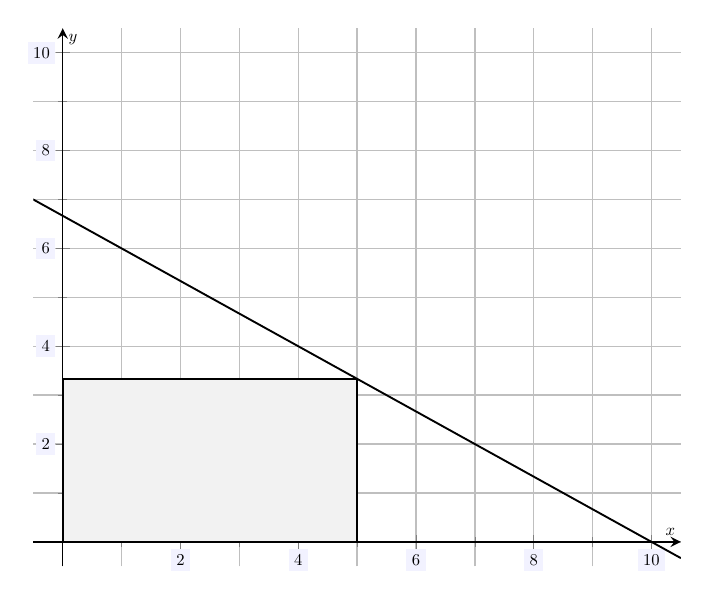
\begin{tikzpicture}[scale=1.2,every node/.style={scale=0.5}]
	\begin{axis}[
	grid=both,
	axis lines=middle,
	ticklabel style={fill=blue!5!white},
	xmin= -0.5, xmax=10.5,
	ymin= -0.5, ymax=10.5,
	xtick={-10,-8,-6,-4,-2,0,2,4,6,8,10},
	ytick={-10,-8,-6,-4,-2,0,2,4,6,8,10},
	minor tick = {-10,-9,...,10},
	xlabel=\(x\),ylabel=\(y\)
	]
	\addplot[line width= 0.02cm,samples=100,domain= -10.5:10.5] ({x},{(20 - 2*x)/3});
	\draw[line width=0.02cm,fill=gray!10] (0,0) -- (5,0) -- (5,10/3) -- (0,10/3) -- (0,0);
	\end{axis}
	\end{tikzpicture}
	}
	\] \pspace

\begin{parts}
\part[5] Find the area of the rectangle shown above. \vfill \vspace{1.1cm}

{\itshape We know that $A= bh$. We know that the base has length 5, i.e. $b= 5$. The height is clearly $f(5)$. But $f(5)= \frac{20 - 2(5)}{3}= \frac{20 - 10}{3}= \frac{10}{3}$. Therefore, we have\dots
	\[
	A= bh= 5 \cdot \dfrac{10}{3}= \dfrac{50}{3} \approx 16.67
	\] \vspace{1.1cm}
}

\part[5] Find $f^{-1}(x)$. \vfill

{\itshape We write $y= \frac{20 - 2x}{3}$. To find $f^{-1}(x)$, we interchange the roles of $x$ and $y$ and solve for $y$. We have\dots
	\[
	\begin{gathered}
	x= \dfrac{20 - 2y}{3} \\
	3x= 20 - 2y \\
	3x - 20= -2y \\
	y= \dfrac{3x - 20}{-2} \\
	y= \dfrac{20 - 3x}{2}
	\end{gathered}
	\]
Therefore, $f^{-1}(x)= \dfrac{20 - 3x}{2}$.}
\end{parts}



% Question 7
\newpage
\question Consider the plot of a relation $\beta$ shown below. 
	\[
	\fbox{
	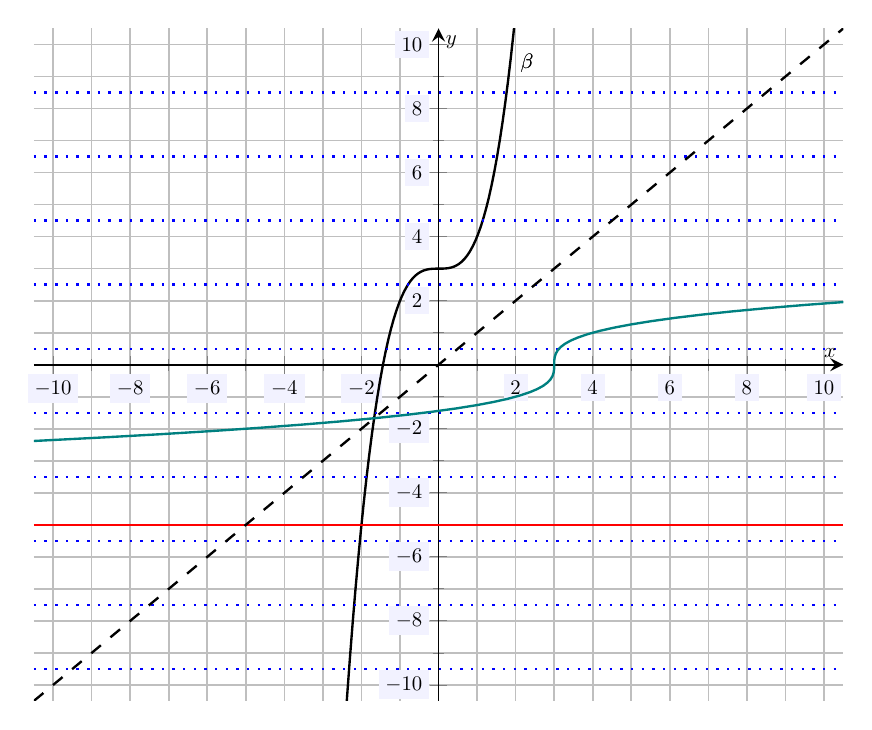
\begin{tikzpicture}[scale=1.5,every node/.style={scale=0.5}]
	\begin{axis}[
	grid=both,
	axis lines=middle,
	ticklabel style={fill=blue!5!white},
	xmin= -10.5, xmax=10.5,
	ymin= -10.5, ymax=10.5,
	xtick={-10,-8,-6,-4,-2,0,2,4,6,8,10},
	ytick={-10,-8,-6,-4,-2,0,2,4,6,8,10},
	minor tick = {-10,-9,...,10},
	xlabel=\(x\),ylabel=\(y\),
	]
	\addplot[line width= 0.02cm,samples=100,domain= -3.5:3.5] ({x},{x^3+3}); \node at (2.3,9.4) {$\beta$}; % Function
	\draw[line width=0.02cm,red] (-10.5,-5) -- (10.5,-5); % Red Line: y= -5
	\foreach \yvalue in {-9.5,-7.5,...,9.5} {
		  \edef\temp{\noexpand\draw[line width=0.02cm,blue,dotted] (-10.5,\yvalue) -- (10.5,\yvalue);} % Dotted blue lines
		  \temp
	}
	\draw[line width=0.02cm,black,dashed] (-10.5,-10.5) -- (10.5,10.5); % Black dotted, y= x
	\addplot[line width= 0.02cm,samples=100,domain= -5:5,teal] ({x^3+3},{x}); \node at (2.3,9.4) {$\beta$}; % Function
	\end{axis}
	\end{tikzpicture}
	}
	\] \pspace

\begin{parts}
\part[2] Is there an $x$ such that $\beta(x)= -5$? Explain. \vfill

{\itshape Observe that the line $y= -5$ (plotted in red) intersects the graph of $\beta(x)$. Therefore, there is an $x$ such that $\beta(x)= -5$. In fact, we can see that $\beta(-2)= -5$.} \vfill

\part[3] Is $\beta$ a function of $x$? Explain. \vfill

{\itshape Yes, $\beta(x)$ is a function of $x$ because it passes the vertical line test; that is, every vertical line intersects the graph of $\beta(x)$ at most once.} \vfill

\part[5] Does $\beta^{-1}(x)$ exist? Justify your answer. If $\beta^{-1}(x)$ doe exist, sketch it on the plot above. \vfill

{\itshape Yes, $\beta^{-1}(x)$ exists because $\beta(x)$ passes the horizontal line test; that is, every horizontal line intersects the graph of $\beta(x)$ at most once (see some plotted as dotted blue lines). We know the graph of $\beta^{-1}(x)$ is the reflection of $\beta(x)$ through the line $y= x$ (plotted as a black dotted line). We have plotted $\beta^{-1}(x)$ above in green.} \vfill
\end{parts}



% Question 8
\newpage
\question \textit{Butte-ane Inc.} is an oil company based out of North Dakota. An engineer at the company reports that the company is shipping the same amount of oil from their reserves each day. They also report that the amount of oil they will have in reserve tanks $d$ days from now, measured in thousands of gallons, is given by $O(d)= 168.438 - 5.3d$. 
	\begin{parts}
	\part[5] Find and interpret the slope of $O(d)$ in the context of the problem. 
	\part[5] Find and interpret the $y$-intercept of $O(d)$ in the context of the problem. 
	\end{parts} \pspace

\tsol
{\itshape
\begin{enumerate}[(a)]
\item We see that the slope of $O(d)$ is $m= -5.3$. We know that $m= \frac{\Delta O}{\Delta d}$. Writing $m= \frac{-5.3}{1}$, we see that for each additional day, the amount of oil decreases by 5.3~thousand gallons; that is, the company ships out 5,300~gallons of oil each day. \pspace

\item We know that the $y$-intercept is $O(d)= 168.438 - 5.3(0)= 168.438 - 0= 168.438$, i.e. $b= 168.438$. But then on day zero, there are 168.438~thousand gallons of oil in the tank; that is, initially, the company has 168,438~gallons of oil in reserve. 
\end{enumerate}
}



% Question 9
\newpage
\question Sanitation workers have finished cleaning Skibidi fountain are refilling it. A hose system is feeding water into the fountain at a constant rate. After 10~minutes, the fountain will require an additional 15,400~gallons of water to fill. But after one hour, the fountain only requires 12,400~gallons. Let $W(t)$ denote the amount of water required to fill the tank after $t$ minutes. 
	\begin{parts}
	\part[5] Explain why $W(t)$ is linear.
	\part[5] Find $W(t)$. 
	\end{parts} \pspace

\tsol
{\itshape
\begin{enumerate}[(a)]
\item The amount of water in the fountain is changing because water is being added to it. But we are told that the water is being added to the fountain at constant rate. But then rate of change in the amount of water in the fountain is constant. Functions with a constant rate of change are linear. Therefore, $W(t)$ must be linear. \pspace

\item From (a), we know that $W(t)= mt + b$. We also know that at the start, the tank required an additional 15,400~gallons of water, i.e. $(0, 15400)$ is a point on the graph of $W(t)$. [From this, we can immediately see that $b= 15400$.] After 1~hour, the tank required 12,400 gallons, i.e. $(1, 12400)$ is a point on the graph of $W(t)$. [From this, we can immediately see that $m= 12400 - 15400= -3,000$.] But then\dots
	\[
	m= \dfrac{\Delta W}{\Delta t}= \dfrac{15400 - 12400}{0 - 1}= \dfrac{3000}{-1}= -3000
	\]
Therefore, $W(t)= -3000t + b$. But we know that when $t= 1$, $W= 12400$. Therefore, we have\dots
	\[
	\begin{gathered}
	W(t)= -3000t + b \\
	W(1)= -3000(1) + b \\
	12400= -3000 + b \\
	b= 15400
	\end{gathered}
	\]
Therefore, $W(t)= -3000t + 15400$. 
\end{enumerate}
}



% Question 10
\newpage
\question[10] Determine whether the following statements are true ($T$) or false ($F$) for all real numbers $x, y, z, a, b$. Mark your answer in the space provided---no justification is necessary. \pvspace{0.5cm}
	\begin{enumerate}[(a)]
	\item \usol{0.65cm}{\itshape T}: $(x^2 + 1)^0= 1$ \vfill
	\item \usol{0.66cm}{\itshape F}: $(x + y)^2= x^2 + y^2$ \vfill
	\item \usol{0.65cm}{\itshape T}: $(x - y)^2= (y - x)^2$ \vfill
	\item \usol{0.66cm}{\itshape F}: $\dfrac{x}{y} + \dfrac{a}{b}= \dfrac{x + a}{y + b}$ \vfill
	\item \usol{0.66cm}{\itshape F}: $\dfrac{\,\,\frac{x}{y}\,\,}{z}= \dfrac{xz}{y}$ \vfill
	\item \usol{0.65cm}{\itshape T}: $\sqrt[3]{-x}= -\sqrt[3]{x}$ \vfill
	\item \usol{0.66cm}{\itshape F}: $\dfrac{x}{y} \cdot \dfrac{a}{b}= \dfrac{xb}{ya}$ \vfill
	\item \usol{0.66cm}{\itshape F}: $\sqrt{x + y}= \sqrt{x} + \sqrt{y}$ \vfill
	\item \usol{0.66cm}{\itshape F}: $\dfrac{x}{y} \cdot \dfrac{a}{b}= \dfrac{xa}{yb}$ \vfill
	\item \usol{0.65cm}{\itshape T}: $(x \cdot y)^a= x^a \cdot y^a$
	\end{enumerate}

\end{questions}
\end{document}